%!TEX root = ../main.tex

\chapter{Anforderungen}

Die Anforderungen an ein Formula Student Fahrzeug werden zum einen durch das 
offizielle Regelwerk der FS Formula und zum anderen durch die Ziele der 
einzelnen Teams festgelegt. Daraus lassen sich dann die Anforderungen an das 
Motion Planning ableiten.

\section{Formula Student Wettbewerb}

Formula Student ist ein internationaler Konstruktionswettbewerb, bei dem jedes 
Jahr von Studententeams von unterschiedlichen Universitäten und Hochschulen 
ein Rennwagen entwickelt, gefertigt und anschließend auf verschiedenen Events 
gegeneinander angetreten wird. Obwohl die Wettbewerbe in vielen verschiedenen 
Ländern stattfinden, orientiert sich diese Arbeit am Regelwerk der Formula Student 
Germany (FSG), da es als Referenz für die Events an denen dieses Team teilnimmt, dient.
Die Wettbewerbe bestehen aus dem Electric Vehicle (EV) Cup und dem Driverless (DV) Cup.
Am EV Cup nehmen Elektrofahrzeuge mit Fahrer teil, während am DV Cup die Fahrzeuge ohne 
Fahrer fahren. Beide Cups bestehen aus mehreren Disziplinen, die sich in statische und 
dynamische Disziplinen unterteilen. Die statischen Disziplinen bewerten hauptsächlich
die Konstruktion und Entwicklung des Fahrzeugs, während bei den dynamischen Disziplinen 
die Fahrleistung auf der Rennstrecke zählt. Ziel ist es hier, die verschiedenen Strecken
in kürzester Zeit zu bewältigen \cite{urlId}.

Ein wichtiger Bestandteil der autonomen Disziplinen ist die Streckenführung, die durch 
Pylonen (engl. Cones) markiert wird. Die linke Begrenzung der Strecke wird durch blaue
Pylonen markiert, die rechte Begrenzung durch gelbe Pylonen. Orangefarbene Pylonen
markieren den Start- und Zielbereich und große orangene Pylonen markieren die Start- 
und Ziellinie. Eine Übersicht der Pylonen nach dem Regelwerg werden in Tabelle 
\ref{tab:cones} dargestellt.

\begin{table}[H]
    \centering
    \begin{tabular}{@{}m{0.15\textwidth} >{\raggedright\arraybackslash}m{0.65\textwidth}@{}}        
        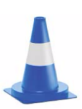
\includegraphics[width=0.1\textwidth]{blue_cone.png} & Kleine blaue Pylonen mit einem weißen Streifen \\
        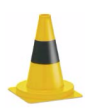
\includegraphics[width=0.1\textwidth]{yellow_cone.png} & Kleine gelbe Pylonen mit einem weißen Streifen \\
        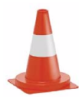
\includegraphics[width=0.1\textwidth]{small_orange_cone.png} & Kleine orange Pylonen mit einem weißen Streifen \\
        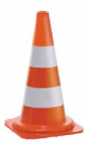
\includegraphics[width=0.1\textwidth]{big_orange_cone.png} & Große orange Pylonen mit zwei weißen Streifen \\
    \end{tabular}
    \caption{Übersicht der Pylonen nach dem Regelwerk \cite{testBuch1}}
    \label{tab:cones}
\end{table}

Sowohl zum EV Cup als auch zum DV Cup gehören die Driverless Disziplinen Acceleration und Skidpad. Zusätzlich 
dazu zählen zum DV Cup die Disziplinen Autocross und Trackdrive.


\subsection{Accel}  

Die Acceleration Disziplin besteht aus einer 75\,m langen Geraden. Ziel ist es, diese Strecke so schnell wie 
möglich zu durchfahren. Nach dem Überqueren der Ziellinie muss das Fahrzeug dann selbstständig bis zum Stillstand 
abbremsen. Abbildung \ref{fig:accel-track} zeigt den schematischen Aufbau der Acceleration Strecke.

\begin{figure}[H]
	\centering
	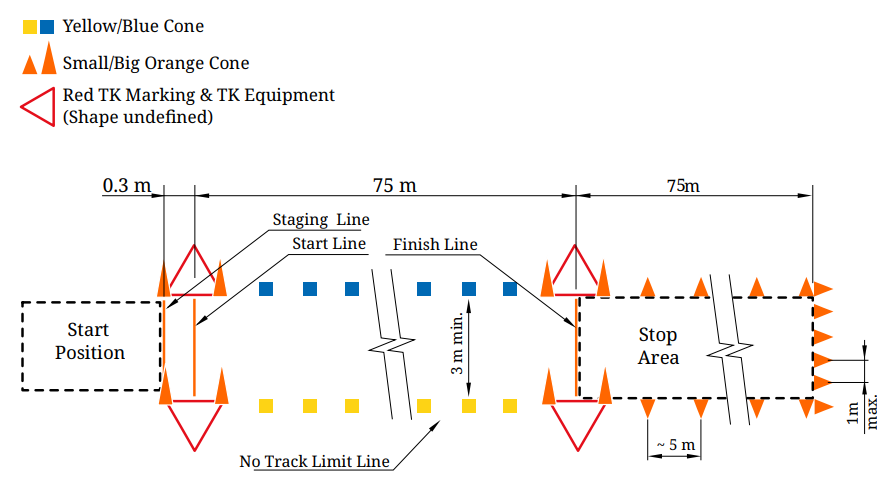
\includegraphics[width=0.8\textwidth]{accel_track.png}
	\caption{Streckenlayout der Acceleration-Disziplin}
	\label{fig:accel-track}
\end{figure}


\subsection{Skidpad}

Die Skidpad Disziplin prüft die Querbeschleunigung des Fahrzeugs. Die Strecke besteht aus zwei Kreisen, die eine
Acht bilden. Als erstes wird die Strecke zweimal in Rechtsrichtung gefahren, wobei nur die Zeit der zweiten Runde 
gemessen wird. Anschließend wird direkt in den anderen Kreis gewechselt und  zwei Runden in Linksrichtung gefahren, 
wobei auch hier nur die Zeit der zweiten Runde gemessen wird. Das Ergebnis der Disziplin entspricht dem Durchschnitt 
der beiden gemessenen Rundenzeiten zuzüglich eventueller Strafen. Abbildung \ref{fig:skidpad-track} zeigt den 
schematischen Aufbau der Skidpad Strecke.

\begin{figure}[H]
	\centering
	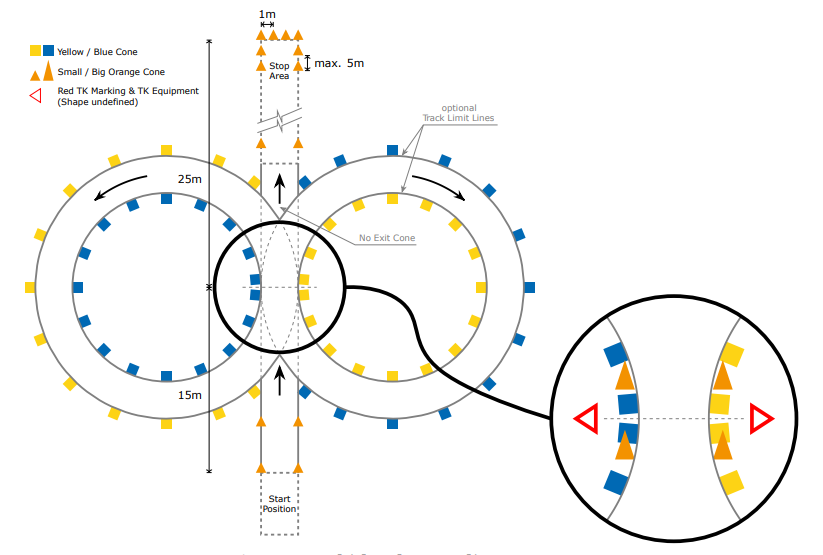
\includegraphics[width=0.8\textwidth]{skidpad_track.png}
	\caption{Streckenlayout der Skidpad-Disziplin}
	\label{fig:skidpad-track}
\end{figure}


\subsection{Autocross und Trackdrive}

Die Autocross und Trackdrive Disziplinen prüfen die Fahrleistung des Fahrzeugs auf einer unbekannten Rennstrecke.
Die Strecke ist mit Pylonen markiert und muss vom Fahrzeug selbstständig durchfahren werden. Die Fahrspur ist 
mindestens 3\,m breit und erstreckt sich über eine Länge von ca. 200 bis 500\,m. Die Start- und Ziellinie ist mit 
orangenen Pylonen markiert und die gleichfarbigen Pylonen auf einer Seite der Strecke haben einen maximalen Abstand
von 5\,m zueinander.

Bei der Autocross Disziplin wird diese Strecke eine Runde gefahren, während bei der Trackdrive Disziplin die 
Strecke zehn Runden gefahren wird. Dementsprechend ist hier eine gute Konsistenz der Fahrleistung über die gesamte
Distanz gefragt. Abbildung \ref{fig:trackdrive-track} zeigt den schematischen Aufbau der Trackdrive Strecke, der sowohl 
für die Autocross als auch für die Trackdrive Disziplin gilt.

\begin{figure}[H]
	\centering
	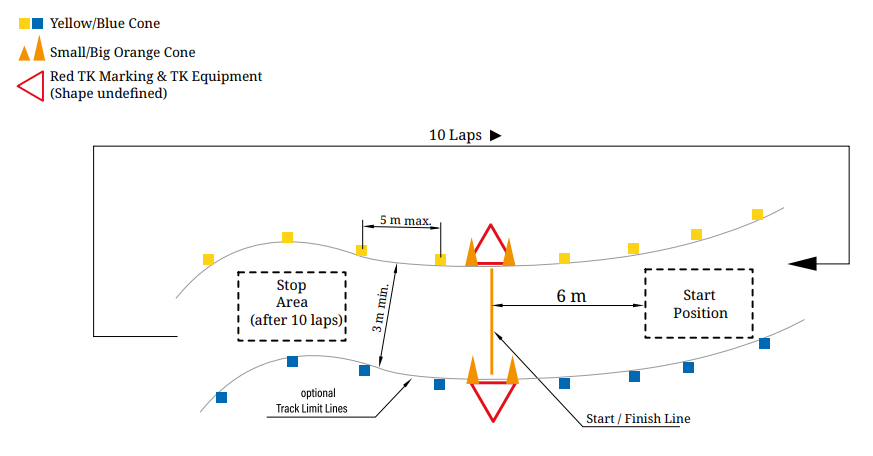
\includegraphics[width=0.8\textwidth]{trackdrive_track.png}
	\caption{Streckenlayout der Trackdrive-Disziplin}
	\label{fig:trackdrive-track}
\end{figure}


\section{Allgemeine Ziele der Saison}
Für die Saison 2027 hat sich das Team DHBW Engineering Stuttgart e.V. das Ziel gesetzt, alle Disziplinen zuverlässig
zu absolvieren. Trotzdem soll die Fahrleistung in den dynamischen Disziplinen weiter verbessert werden, um eine 
Platzierung unter den Top 5 im DV Cup zu erreichen. Um dieses Ziel zu erreichen, wurden Zielwerte für die einzelnen
Disziplinen festgelegt, die in Tabelle \ref{tab:goals} dargestellt werden. Diese Zielwerte basieren auf Erfahrungswerten
aus den vergangenen Saisons, eine solche Platzierung realistisch erscheinen zu lassen. Auf die genaue Herleitung 
dieser Zielwerte wird im Rahmen dieser Arbeit verzichtet.

\medskip
\medskip

\begin{table}[H]
	\centering
	\begin{tabular}{|l|c|c|}
		\hline
		Disziplin & Zielzeit & Zielgeschwindigkeit \\
		\hline
		Accel & 3,6 &  \\
		Skidpad & 5,0 &  \\
		Autocross &  & 60\% des Fahrzeuglimits \\
		Trackdrive &  & 60\% des Fahrzeuglimits \\
		\hline
	\end{tabular}
    \caption{Zielwerte für die einzelnen Disziplinen}
    \label{tab:goals}
\end{table}

\section{Ziele für das Motion Planning}